\documentclass[12pt,letterpaper,final]{report}
\usepackage[utf8]{inputenc}
\usepackage{amsmath}
\usepackage{amsfonts}
\usepackage{amssymb}
\usepackage{amsthm}
\renewcommand\qedsymbol{$\blacksquare$}
\usepackage{enumerate}
\usepackage{hyperref}
\usepackage{pdfpages}
\usepackage{graphics}
\usepackage{graphicx}
\usepackage{tikz}
\usepackage{tikz-qtree}
\usetikzlibrary{automata,arrows}



%\author{Marius Zimand}

\begin{document}


\fbox{
\vbox{
\begin{flushleft}
Anna Cooper, John Smith, Nick Curly \\  % authors' names
COSC 999 \\  %class
1/31/2018\\  % date
\end{flushleft}
\center{\Large{\textbf{Assignment 1}}}
%\end{mdframed}
} % end vbox
} % end fbox
\vline


\noindent\textbf{Problem 1:}  Here is the solution for problem 1.

Mathematical text is written like this $a+b = c$.

This is how we can have subscripts and superscripts: $a^2 + b^2 = c^2 + d_1$.

For union of sets, write $A \cup B$; for intersection $A \cap B$; the empty set is denoted $\emptyset$.




Greek letters are easy to write: $\alpha$, $\beta$, $\gamma$, $\theta$, $\Theta$, $\omega$, $\Omega$, and so on. 

See \url{https://artofproblemsolving.com/wiki/index.php/LaTeX:Symbols} for a large list of latex symbols.

This is how we can write math equations on a separate line:
\[
a+b = c^2 + \log n. 
\]

This is how we can write math equations on a separate line, which include normal text
\[
a+b = c^2 + \log n. \mbox{    (Joe's equation).}
\]

This is how we can write multi-line math equations on a separate line:
\[
\begin{array}{ll}
a+b & = c^2 + \log n \\
&\leq 5d + \sin x \\
& = A.
\end{array}
\]
Matrices can be written like this:
\[
A = 
\begin{pmatrix}
1 & a & b \\
2 & a^2 & b^3 \\
3 & a_3 & b_5
\end{pmatrix}
\]
\bigskip

This is how to make a table:

\medskip

\begin{tabular}{|c|c|c|}
\hline
$\delta$ & $a$ & $x$ \\
\hline
$q_{1}$ & $q_{1}$ & $ b$ \\
$q_{2}$ & $q_{1}$ & $ c$ \\
$q_{3}$ & $q_{2}$ & $ b$ \\
$q_{4}$ & $q_{3}$ & $ c$ \\
$q_{5}$ & $q_{4}$ & $ b$ \\
\hline
\end{tabular}
\medskip

This is how to draw the diagram of an automaton:
\medskip

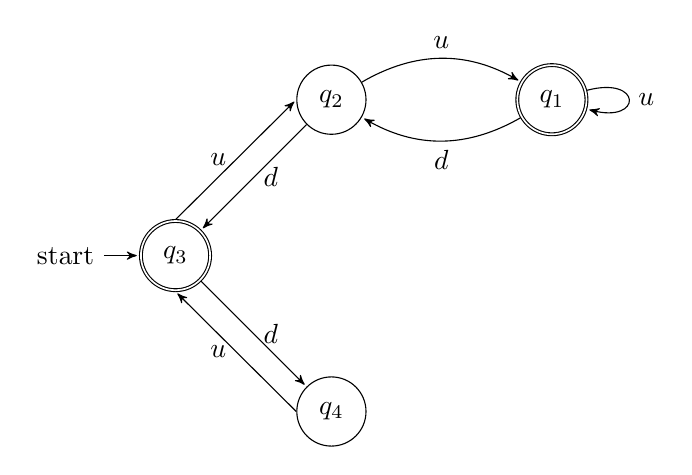
\begin{tikzpicture}[>=stealth',shorten >=1pt,auto,node distance=2.8cm]]

  \node[initial, state, accepting] (3) {$q_{3}$};
  \node[state] (2) [above right of=3] {$q_{2}$};
  \node[state] (4) [below right of=3] {$q_{4}$};
  \node[state, accepting] (1) [right of=2] {$q_{1}$};
 
  
  \path[->]
    (3.north) edge [left] node {$u$} (2.west)    
    (2) edge [right] node {$d$} (3)
    
    (3) edge [right] node{$d$} (4)
    (4.west) edge [left] node {$u$} (3.south)
    
    (2) edge [bend left] node[above] {$u$} (1)
    (1) edge [loop right] node {$u$} (1)
    (1) edge [bend left] node[below] {$d$} (2)
       ;  
\end{tikzpicture}

This is how to draw an arbitrary graph using a package called TikZ.
\medskip


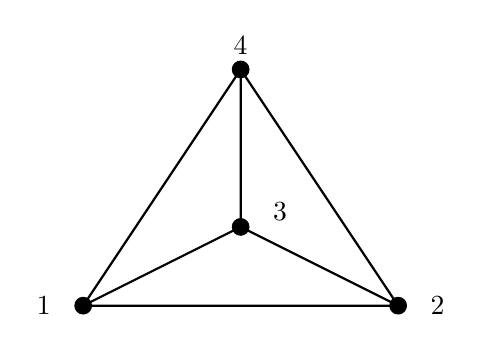
\begin{tikzpicture}
%% vertices
\draw[fill=black] (0,0) circle (3pt);
\draw[fill=black] (4,0) circle (3pt);
\draw[fill=black] (2,1) circle (3pt);
\draw[fill=black] (2,3) circle (3pt);
%% vertex labels
\node at (-0.5,0) {1};
\node at (4.5,0) {2};
\node at (2.5,1.2) {3};
\node at (2,3.3) {4};
%%% edges
\draw[thick] (0,0) -- (4,0) -- (2,1) -- (0,0) -- (2,3) -- (4,0) -- (2,1) -- (2,3);
\end{tikzpicture}

This should be pretty self-explanatory. The ordered pairs in parentheses are all simply coordinates in the plane.


The edges are drawn by taking a walk through the graph, using each edge exactly once.
You can do much fancier things in TikZ, but this should at least get you started.




\bigskip

To make latex produce the text exactly how we type, we can use the verbatim environment. This is useful for example to write an algorithm in pseudo-code. Below is a short example.

\begin{verbatim}
s = 0
for i going from 1 to n

   s= s+ a[i]

end-for
\end{verbatim}

To append in the  latex file the Java source code and the screenshots, you can print them  as a pdf file (placed in the same folder) and then include them  in the latex file with 
\begin{verbatim}
\includepdf[pages=-,pagecommand={},width=\textwidth]{file.pdf}

\end{verbatim}
To append in the  latex file a .jpg file (for a photo), use 
\begin{verbatim}
\includegraphics[width=\linewidth]{photo.jpg}

\end{verbatim}




\noindent\textbf{Problem 2:} Here is the solution for problem 2.....





\bigskip

\noindent\textbf{Problem 3:} Here is the solution for problem 3. ...


\bigskip

\noindent\textbf{Problem 4:}  Here is the solution for problem 4. ...

\end{document}